\documentclass[conference]{IEEEtran}
% \IEEEoverridecommandlockouts
% The preceding line is only needed to identify funding in the first footnote. If that is unneeded, please comment it out.
\usepackage{cite}
\usepackage{amsmath,amssymb,amsfonts}
\usepackage{algorithmic}
\usepackage{graphicx}
\usepackage{textcomp}
\usepackage[center]{caption}
\usepackage{comment}
\usepackage{xcolor}
\def\BibTeX{{\rm B\kern-.05em{\sc i\kern-.025em b}\kern-.08em
    T\kern-.1667em\lower.7ex\hbox{E}\kern-.125emX}}
\usepackage{tikz}
\usetikzlibrary{shapes,arrows,positioning,calc}

\tikzset{
block/.style = {draw, fill=white, rectangle, minimum height=3em, minimum width=3em},
tmp/.style  = {coordinate}, 
sum/.style= {draw, fill=white, circle, node distance=1cm},
input/.style = {coordinate},
output/.style= {coordinate},
pinstyle/.style = {pin edge={to-,thin,black}
}
}

\begin{document}

\title{Identification of Multiple Copy-move Attacks in Digital Images using FFT and CNN}

%\title{Detection of Copy-move Image Forgery using FFT and Convolutional Neural Networks}

%\title{Combination of FFT and Convolutional Neural Networks to Detect Copy-move Image Forgery}

\makeatletter
\newcommand{\linebreakand}{%
  \end{@IEEEauthorhalign}
  \hfill\mbox{}\par
  \mbox{}\hfill\begin{@IEEEauthorhalign}
}
\makeatother
\renewcommand\IEEEkeywordsname{Keywords}

\author{\IEEEauthorblockN{Gokul Nair}
\IEEEauthorblockA{\textit{Department of Electronics and Telecommunications} \\
\textit{Sardar Patel Institute of Technology}\\
Mumbai-58, India \\
gokul.nair@spit.ac.in}
\and
\IEEEauthorblockN{Kaustubh Venkatesh}
\IEEEauthorblockA{\textit{Department of Electronics and Telecommunications} \\
\textit{Sardar Patel Institute of Technology}\\
Mumbai-58, India \\
kaustubh.v@spit.ac.in}
\linebreakand
\IEEEauthorblockN{Dipankar Sen}
\IEEEauthorblockA{\textit{Department of Electronics and Telecommunications} \\
\textit{Sardar Patel Institute of Technology}\\
Mumbai-58, India \\
dipankar.sen@spit.ac.in}
\and
\IEEEauthorblockN{Reena Sonkusare}
\IEEEauthorblockA{\textit{Department of Electronics and Telecommunications} \\
\textit{Sardar Patel Institute of Technology}\\
Mumbai-58, India \\
reena\_kumbhare@spit.ac.in}
}

\maketitle

\begin{abstract}
Copy-move forgery is an image manipulation technique wherein significant elements are added or removed from the image to spread misinformation. These forged images have flooded the internet owing to easily accessible image editing software. Copy-move attacks distort edges around the manipulated elements and thus can be detected by analyzing these edges. Traditional detection methods utilize algorithms like Cosine Transform, Scale-invariant Feature Transform, and Convolution Neural Networks (CNN), which have varying levels of accuracy and fail when there are multiple copy-move attacks in the image. Since edge detection and analysis are critical steps, performing Preliminary Edge Detection on the images proves effective. This study proposes Fast Fourier Transform (FFT) to perform preliminary edge detection on the images used to train the CNN model. The proposed algorithm that combines FFT and CNNs achieves enhanced testing accuracy of 95.91\%, low validation loss of 0.252, and performs exceptionally well with multiple copy-move attacks.
% Copy-move forgery is an image manipulation technique wherein significant elements are added or removed from the image to spread false information. These forged images have flooded the internet due to the ease of performing such manipulations using accessible image editing software. However, copy-move attacks result in distortion of edges around the manipulated elements. Thus, these manipulations can be detected by analyzing the edges of elements in the image. Traditional methods for detecting such forgeries include edge detection algorithms like Fourier Transform, Scale-invariant Feature Transform (SIFT), and Convolution Neural Networks (CNN), which have varying levels of accuracy. These methods fail when there are multiple copy-move attacks in the image. Since edge detection and analysis are critical steps in identifying manipulated images, performing Preliminary Edge Detection on the input images proves effective. This study proposes an algorithm that uses Fast Fourier Transform (FFT) to perform preliminary edge detection on the input dataset which is used to train the proposed CNN model. The proposed algorithm which uses a combination of FFT and CNNs achieves enhanced testing accuracy of 95.91 \%  and a low validation loss of 0.252. The model performs exceptionally well with images containing multiple copy-move attacks.

\end{abstract}
\begin{IEEEkeywords}
Copy-move forgery, Fast Fourier Transform, Image edge detection, Convolutional Neural Networks
\end{IEEEkeywords}

\section{Introduction}
Every day, users upload more than 1.8 billion digital images to the internet. With the widespread adoption of smartphones and the internet, this number will surely increase. While the advancement of imaging technology has benefited many spheres of society, image manipulation and forgery continue to remain an issue. Forwarding of modified images shared over social media is growing at unmanageable rates and tends to have real-life implications. Fig. \ref{modi} shows an instance of a copy-move forged image used to spread misinformation. Moreover, the development of powerful image editing tools such as Photoshop has made manipulation of images even more effortless. Thus, detection and classification of such manipulated images is imperative. 

Forgers use various image manipulation methods. These include image splicing, Copy-move forgery, and image retouching \cite{b1} \cite{b16}. Copy-move forgery is the process by which complete elements are added or removed from the original image. Images manipulated using this method are believable as modern tools allow seamless integration of such components. Detection algorithms use the fact that the edges of manipulated elements in such images are distorted \cite{b2}. These algorithms use various tools such as Fourier Transforms, Cosine Transforms, Convolutional Neural Networks (CNNs), etc. \cite{b1} to detect and classify manipulated images, which have varied levels of success. 

\begin{figure}[htpb]
\centerline{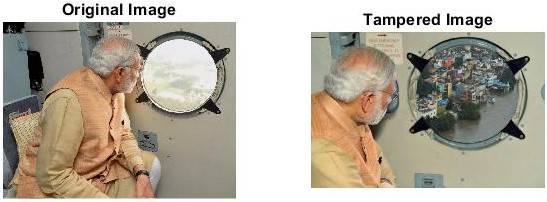
\includegraphics[width=8cm]{modi.jpg}}
\caption{Real instance of a copy-move attack \cite{b14}}
\label{modi}
\end{figure}

There are various datasets created to aid the development of such algorithms. This study plans to use Fast Fourier Transform (FFT) \cite{b10} combined with CNNs to improve the success rate of copy-move forgery detection.

\section{Related Work}
Many studies have advocated using transformation functions such as Scale-invariant feature transform (SIFT), Fourier and Cosine transforms \cite{b19}, and convolution to perform edge detection on images \cite{b1}. \cite{b2} advocates the use of a 2-dimensional Fourier Transform to detect copy-move forgery with an accuracy of 87 \%. \cite{b3} proposes CNN models to detect copy-move forgeries with 90 \% accuracy. \cite{b4} proposes the use of SIFT as a solution and also provides a dataset to help develop copy-move forgery detection techniques. \cite{b5} introduces and compares various other methods to perform detection and also provides a reliable image dataset for development. \cite{b6} highlights various methods to detect attacks such as Support Vector Machines (SVM), Markov Chains, Wavelet Decomposition and also proposes a CNN model. \cite{b8} proposes the use of Singular value decomposition (SVD). \cite{b20} uses a localization algorithm for detecting duplicated regions in the forged image. \cite{b18} proposes the Speed Up Robust Features (SURF) algorithm to detect manipulations.

While these methods are effective in detecting copy-move forgery to a reasonable extent, they fail to correctly classify images where there are multiple copy-move attacks. Moreover, the studies discussed use restricted datasets which results in poor performance due to underfitting of the models. The main contribution of this study is the identification and use of FFT to perform preliminary edge detection which helps the CNN algorithm perform better with larger datasets and multiple copy-move attacks. This helps improve the success rate of classification.

The organization of the paper is as follows. Section III lays out the algorithm and design of the CNN model used. Section IV delineates the outcome of the study and explains why the model is better than its precursors. Section V concludes the study and summarizes the importance of forgery detection and finding an efficient mechanism.

\section{Methodology}
Copy-move forgery detection is based on the fact that the manipulated images have distorted edges around the elements added to or deleted from the image. Thus, edge detection is an important step in classifying such images. The most effective method for performing edge detection is the Fourier Transform. This study uses FFT to perform preliminary edge detection to aid the training of the proposed CNN. The CNN classification algorithm relies on feature extraction and edge detection using convolution. It thus achieves improved accuracy as the images in the dataset already have clearly defined edges. This allows the study to reduce the number of convolution layers in the CNN model without reducing accuracy while improving efficiency. Fig. \ref{flowchart} depicts the flowchart of the proposed method.

\begin{figure}[htpb]
\centerline{
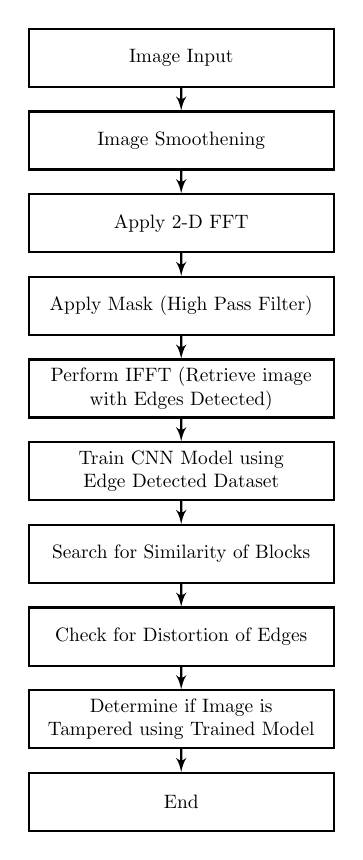
\begin{tikzpicture}[thick,scale=0.50, every node/.style={scale=0.7},text width=35ex, align=center,node distance=1.5cm,>=latex']
    \node [block, name=input] (input) {Image Input};
    \node [block, below of=input] (smooth) {Image Smoothening};
    \draw [->] (input) -- (smooth);
    \node [block, below of=smooth] (fft) {Apply 2-D FFT};
    \draw [->] (smooth) -- (fft);
    \node [block, below of=fft] (mask) {Apply Mask (High Pass Filter)};
    \draw [->] (fft) -- (mask);
    \node [block, below of=mask, align=center] (ifft) {Perform IFFT (Retrieve image \\ with Edges Detected)};
    \draw [->] (mask) -- (ifft);
    \node [block, below of=ifft, align=center] (cnn) {Train CNN Model using Edge Detected Dataset};
    \draw [->] (ifft) -- (cnn);
    \node [block, below of=cnn, align=center] (sim) {Search for Similarity of Blocks};
    \draw [->] (cnn) -- (sim);
    \node [block, below of=sim, align=center] (dist) {Check for Distortion of Edges};
    \draw [->] (sim) -- (dist);
    \node [block, below of=dist, align=center] (pred) {Determine if Image is\\ Tampered using Trained Model};
    \draw [->] (dist) -- (pred);
    \node [block, below of=pred, align=center] (end) {End};
    \draw [->] (pred) -- (end);
\end{tikzpicture}}
\caption{Flowchart of the proposed method}
\label{flowchart}
\end{figure}

\begin{comment}
\begin{figure}[htpb]
\centerline{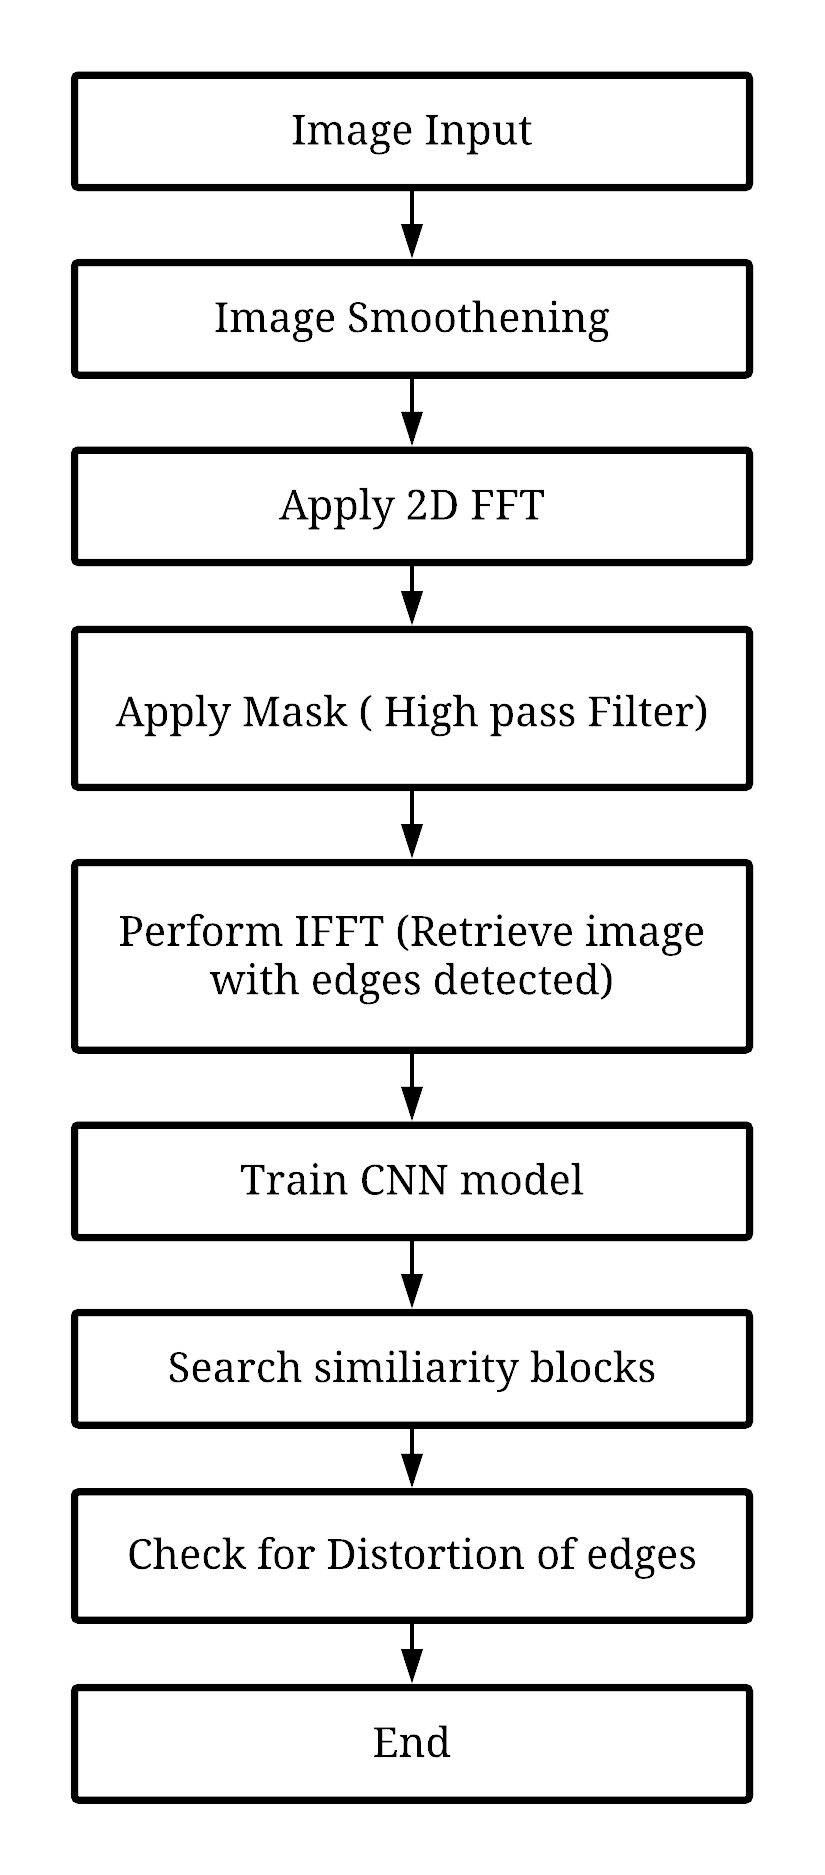
\includegraphics[scale=0.45]{block diagram-2.png}}
\caption{Flowchart of the proposed method \cite{b14}}
\label{flowchart}
\end{figure}
\end{comment}

\subsection{Experimental Setup}
The study uses the Spyder and Google Colaboratory development environments based on Python for performing FFT and training the CNN models. The Python libraries used include OpenCV, NumPy, Pandas, Matplotlib, Tensorflow, and Keras.  

\subsection{Experimental Dataset}
The study derives its dataset from multiple sources. These include image datasets created especially to aid the development of copy-move forgery detection techniques. Images from various studies \cite{b4}  \cite{b5} \cite{b7} were randomly selected and combined to form a comprehensive dataset containing 1000 images, with 500 being originals and the rest being their tampered copies. The images in the dataset include samples with single as well as multiple copy-move attacks to make the dataset exhaustive. Fig. \ref{tampered} shows one of the sample pairs from the dataset.

\begin{figure}[htpb]
\centerline{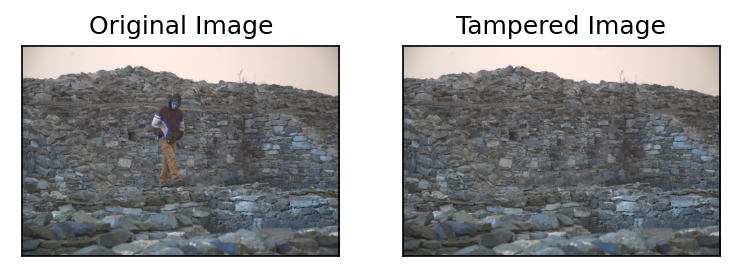
\includegraphics[width = 9cm]{tamp_up.png}}
\caption{Example of image manipulation using copy-move forgery}
\label{tampered}
\end{figure}

\subsection{Preliminary Edge Detection}
The study uses the Fast Fourier Transform (FFT) algorithm \cite{b10}, an efficient implementation of the Discrete Fourier Transform, which is used to determine the frequency domain representation of a signal. The proposed algorithm performs FFT (2-dimensional 64 point) on the input images to obtain the magnitude spectrum. It then applies a mask in the form of a High Pass Filter (HPF) to retain only the desired frequencies and perform edge detection \cite{b15}. It then performs Inverse Fast Fourier Transform (IFFT) on the signal obtained to retrieve the image with highlighted edges. The dataset of images retrieved after edge detection forms the input training data for the CNN model. Fig. \ref{fft} shows the effect of FFT on the input image as the edges are clearly visible.

\begin{figure}[htpb]
\centerline{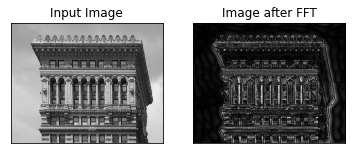
\includegraphics[width = 9cm]{fft.png}}
\caption{Output after performing edge detection using FFT}
\label{fft}
\end{figure}

\subsection{Convolutional Neural Networks}
CNN is a deep learning algorithm that utilizes the convolution of the image matrix using an edge detection kernel \cite{b11}. Convolution preserves the spatial relationship between pixels. Image classification applications often utilize CNN models. The model used is a sequential model with a two-dimensional convolution layer with input size (None, 224, 224, 3).  The model has a max-pooling layer, which reduces the spatial size of the convoluted features. This reduces the computational time taken to train the model. A flattening layer follows, which converts the polled features into a single column. Dense layers add non-linear characteristics to the model, making it more universal. The model employs Adam optimizer \cite{b9} with a learning rate of 10$^{-3}$. Loss is the quantity that the model seeks to reduce during training. The loss parameter for the model is categorical cross-entropy \cite{b13}. Fig. \ref{model} shows the structure of the designed model. 

\begin{figure}[htpb]
\centerline{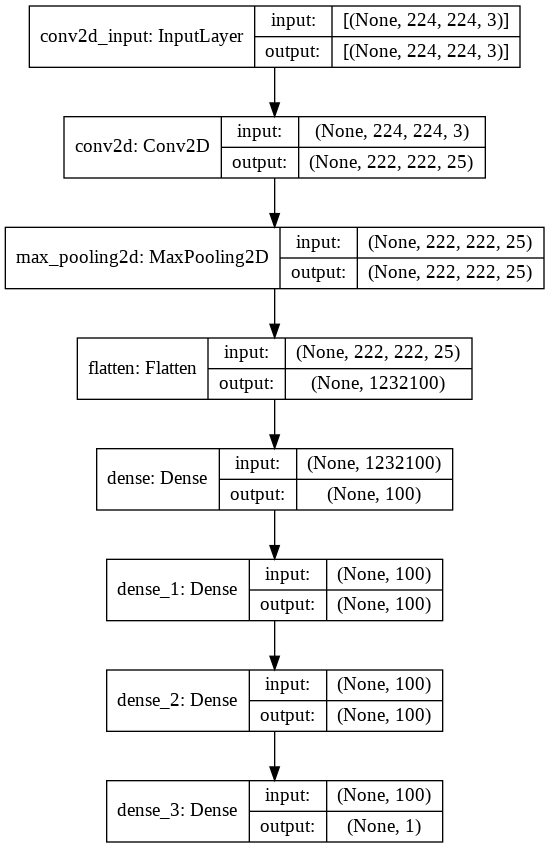
\includegraphics[scale = 0.32]{model.png}}
\caption{Structure of the CNN model}
\label{model}
\end{figure}

The study trains the model using the edge detected image dataset. The study randomly splits the dataset into two sets (80 percent train and 20 percent validation). The split sets contain a mix of original and tampered images labeled as 0 for original and 1 for tampered images. Studies can modify the input 'conv2d' layer of the proposed model to be the output layer of an extensive pre-trained model such as VGG16 or Resnet. 


\section{Results}
This section presents the metrics used to evaluate the model's efficiency of classification. The metrics used for the CNN model are Accuracy, Area Under Curve (AUC) \cite{b12}, Recall, Precision, and Loss \cite{b17}. Accuracy is the best metric for assessing the efficiency of binary classification algorithms. The equation for binary accuracy is :

\begin{equation}
   Accuracy = \frac{TP +TN}{TP +TN + FP +FN}
\end{equation}
where,
\newline
TP = True Positive , TN = True Negative \newline 
FP = False Positive , FN = False Negative

\begin{figure}[htpb]
\centerline{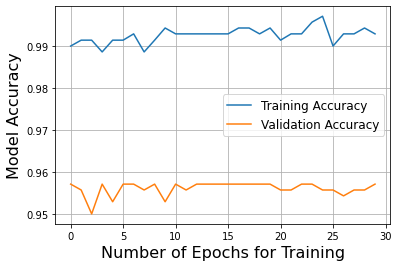
\includegraphics[width=8cm]{accuracy.png}}
\caption{Training and Validation Accuracy plots of the CNN model using the Edge Detected Dataset}
\label{accuracy}
\end{figure}

Fig. \ref{accuracy} depicts the model accuracy for training and validation datasets over 30 epochs. The accuracy increases as the number of epochs increases. Fig. \ref{auc} shows the plot of AUC for training and validation dataset for 30 epochs. An AUC closer to 1, indicates good separability. Fig. \ref{precision} and Fig. \ref{recall} show the precision and recall curves of the model respectively. Improving precision usually reduces recall and vice-versa. Loss characterizes how poorly the model performs during prediction. Fig. \ref{loss} depicts the loss curves for the model. Loss values closer to 0 indicate a better model.

\begin{figure}[htpb]
\centerline{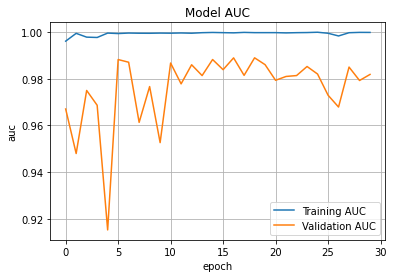
\includegraphics[width=8cm]{auc.png}}

\caption{Training and Validation AUC plot of the CNN model using the Edge Detected Dataset}
\label{auc}
\end{figure}

\begin{figure}[htpb]
\centerline{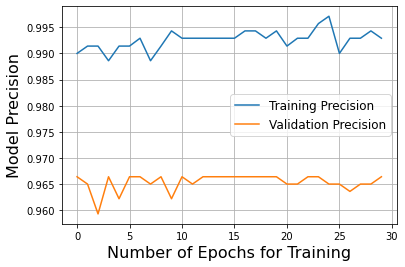
\includegraphics[width=8cm]{precision.png}}
\caption{Training and Validation Precision plot of the CNN model using the Edge Detected Dataset}
\label{precision}
\end{figure}


\begin{figure}[htpb]
\centerline{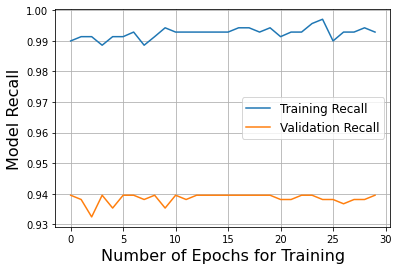
\includegraphics[width=8cm]{recall.png}}
\caption{Training and Validation Recall plot of the CNN model using the Edge Detected Dataset}
\label{recall}
\end{figure}

\begin{figure}[htpb]
\centerline{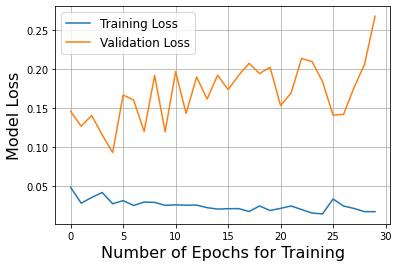
\includegraphics[width=8cm]{loss.png}}
\caption{Training and Validation Loss plot of the CNN model using the Edge Detected Dataset}
\label{loss}
\end{figure}

The confusion matrix is a visual method to evaluate model performance. It indicates the accuracy of classification based on predicted and actual values by the model. Fig. \ref{confusion} shows the confusion matrix for the model. The model correctly predicts 90 images as original and misclassifies 5 images as tampered. It accurately classifies 102 images as tampered and misclassifies 3 tampered images as original.

\begin{figure}[htpb]
\centerline{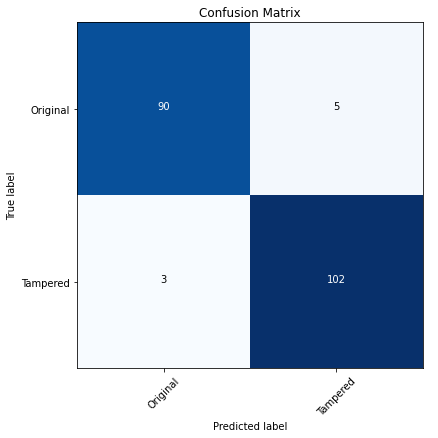
\includegraphics[scale=0.45]{confusion.png}}
\caption{Confusion matrix of the Edge Detected Validation Dataset}
\label{confusion}
\end{figure}

\begin{table}[htpb]
\caption{\label{tab:res}Performance metrics of the CNN model using the Edge Detected Dataset}
\centering
\resizebox{250pt}{!}{%
\begin{tabular}{|c|c|c|c|c|c|}
\hline
Data & Accuracy & AUC & Recall & Precision & Loss \\  
\hline
Training & 99.29 \% & 0.999  &  0.993 & 0.987 & 0.0167 \\
\hline
Validation & 95.91 \% & 0.989  & 0.9395  &  0.9664 & 0.252 \\
\hline
\end{tabular}
}
\end{table}

Table I summarizes the performance parameters of the model. The model achieves high AUC, recall, and precision. Loss for both training and validation datasets is very low. These values verify that the model is not overfitting, and the features of the model apply to images outside the dataset without loss of accuracy. 

\begin{table}[htpb]
\centering
\caption{\label{tab:acc} Comparative Analysis of Accuracies of various Detection Algorithms}
\resizebox{240pt}{!}{%
\begin{tabular}{|c|c|}
\hline
Method & Accuracy \\  
\hline
Scale-invariant feature transform \cite{b4} & 79.41 \% \\
\hline
2-Dimensional Fourier Transform \cite{b2} & 86.57\% \\ 
\hline
Singular Value Decomposition (SVD) \cite{b8} & 87.8 \% \\
\hline
Convolutional Neural Network \cite{b3} & 90.42 \% \\
\hline
FFT + CNN (Proposed Method) & 95.91 \%  \\ 
\hline
\end{tabular}
}
\end{table}

Table II summarizes the accuracies of various methods of copy-move forgery detection. SIFT method \cite{b4} achieves an accuracy of 79.41 \% using the same dataset. Implementing 2-Dimensional FFT \cite{b2} yields 86.57 \% accuracy while SVD \cite{b8} achieves an accuracy of 87.8 \%.  The CNN proposed by \cite{b3} achieves a maximum accuracy of 90.42 \%. The proposed method combines FFT with CNN and achieves an accuracy of 95.91\%, an improvement of 5.5 \%. 


CNNs use convolution as their first step, wherein the edges of the elements in the image are identified using feature mapping and used to train the neural network. The proposed method achieves improved performance as the input images for the CNN already have clearly defined edges. The transformed images reduce the amount of computation required to detect elements at each epoch of training. This also reduces the possibility of errors while performing convolution on the image. This improves the overall accuracy of the model. The model performs well with instances of multiple copy-move attacks considering the composition of the validation dataset which contains a comprehensive mix of original and tampered images with single and multiple copy-move attacks. 

\section{Conclusion}
As image editing technologies become more powerful and accessible, the development of corresponding methods to detect such manipulations is imperative to curb the spread of misinformation. While these manipulations may not be apparent to the human eye, appropriate algorithms can effectively identify such images. This study proposes a method to detect copy-move forgery, an effective and widespread image manipulation technique. The study compares various methods developed to solve this problem, all of which assess the distortion in the edges of elements in manipulated images. The dataset used by the study contains a comprehensive and balanced set of image samples from various sources with single as well as multiple copy-move attacks. CNNs perform the best as they use convolution for edge detection, using which the subsequent neural network layers are trained. Preliminary edge detection on the input images is effective as the clearly defined edges of these images help the CNN algorithm perform better. The study uses FFT to perform preliminary edge detection on the image dataset. The edge detected dataset is then used to train the proposed CNN model. The study analyses the developed model using performance metrics like accuracy, AUC, precision, recall, loss, and confusion matrix. The proposed method achieves an improved accuracy of 95.91 \%. The CNN model developed also achieves a high AUC of 0.99 and a low loss value of 0.25. Future studies can consider other edge detection algorithms in combination with CNNs. Studies can use the concept of Transfer Learning and pre-trained models like Inception and Resnet to improve the success rate. 

% Studies can also extend the proposed method to other forms of image manipulation.


\begin{thebibliography}{00}\bibitem{b1}Basavarajappa, Shwetha B \& Sathyanarayana, “ Digital image forgery detection techniques: a survey,” \textit{ACCENTS Transactions on Information Security}, 2016,vol. 2, pp. 22-31,  doi:10.19101/TIS.2017.25003.

\bibitem{b16}Birajdar, G. K., \& Mankar, V. H, “Digital image forgery detection using passive techniques: A survey. Digital Investigation,” 2013, vol. 10(3), pp. 226–245. doi: 10.1016/j.diin.2013.04.007.

\bibitem{b2}Ketenci, Seniha \& Ulutas, Guzin, “Copy-move forgery detection in images via 2D-Fourier Transform,” 2013, pp.813-816, doi:10.1109/TSP.2013.6614051. 

\bibitem{b14}BBC News, “Chennai floods: Edited Modi photo sparks online mockery,” Dec.2015, https://www.bbc.com/news/world-asia-india-34991822 

\bibitem{b10}E. O. Brigham and R. E. Morrow, “The fast Fourier transform,”  \textit{IEEE Spectrum}, vol. 4, no. 12, pp. 63-70, Dec. 1967, doi: 10.1109/MSPEC.1967.5217220.

\bibitem{b19}Alkawaz, M.H., Sulong, G., Saba, T. et al., “Detection of copy-move image forgery based on discrete cosine transform,”\textit{ Neural Computing and Applications}, 2016, vol. 30(1), pp.183–192. doi:10.1007/s00521-016-2663-3.

\bibitem{b3}Y. Abdalla, M. Iqbal, and M. Shehata, “Convolutional Neural Network for Copy-Move Forgery Detection,” Symmetry, vol. 11, no. 10, pp. 1280, Oct. 2019. doi: 11. 1280. 10.3390/sym11101280.

\bibitem{b4} I. Amerini, L. Ballan, R. Caldelli, A. Del Bimbo, G. Serra, 
“A SIFT-based forensic method for copy-move attack detection and transformation recovery”, \textit{IEEE Transactions on Information Forensics and Security},2011, vol. 6, issue 3, pp. 1099-1110. 

\bibitem{b5}V. Christlein, C. Riess, J. Jordan, C. Riess, E. Angelopoulou, “An Evaluation of Popular Copy-Move Forgery Detection Approaches", 
\textit{IEEE Transactions on Information Forensics and Security}, 2012, vol. 7, no. 6, pp. 1841-1854,  doi: 10.1109/TIFS.2012.2218597.

\bibitem{b6}Agarwal, Shruti \& Fan, Wei \& Farid, Hany, “A Diverse Large-Scale Dataset for Evaluating Rebroadcast Attacks," 2018, vol. 2018, pp.1997-2001. doi: 10.1109/ICASSP.2018.8462205.

\bibitem{b8}Kashyap, Abhishek \& Agarwal, Megha \& Gupta, Hari, “ Detection of Copy-move Image forgery using SVD and Cuckoo Search Algorithm," \textit{International Journal of Engineering and Technology(UAE)},2017, vol.7, doi: 10.14419/ijet.v7i2.13.11604. 

\bibitem{b20}Jaberi, M., Bebis, G., Hussain, M. et al., “Accurate and robust localization of duplicated region in copy–move image forgery,"\textit{Machine Vision and Applications},2014, vol. 25, pp. 451–475, doi: https://doi.org/10.1007/s00138-013-0522-0.

\bibitem{b18}X. Bo, W. Junwen, L. Guangjie and D. Yuewei, “Image Copy-Move Forgery Detection Based on SURF," \textit{2010 International Conference on Multimedia Information Networking and Security, Nanjing, China}, 2010, pp. 889-892, doi: 10.1109/MINES.2010.189.

\bibitem{b7}D.-T. Dang-Nguyen, C. Pasquini, V. Conotter, G. Boato, “ RAISE – A Raw Images Dataset for Digital Image Forensics,"\textit{ ACM Multimedia Systems, Portland, Oregon}, March 18-20, 2015

\bibitem{b15}A. Sinha, “Edge detection in images using Fourier Transform,” 2018, https://akshaysin.github.io/fourier\_transform.html\#.YGcLo7DitPZ.

\bibitem{b11}S. Albawi, T. A. Mohammed and S. Al-Zawi, “Understanding of a convolutional neural network," \textit{2017 International Conference on Engineering and Technology (ICET), Antalya, Turkey}, 2017, pp. 1-6, doi: 10.1109/ICEngTechnol.2017.8308186.

\bibitem{b9}Diederik P. Kingma, Jimmy Ba “Adam: A Method for Stochastic Optimization” arXiv:1412.6980 [cs.LG] 30 Jan 2017.

\bibitem{b13}Zhilu Zhang and Mert R. Sabuncu, “Generalized cross entropy loss for training deep neural networks with noisy labels," \textit{ 32nd International Conference on Neural Information Processing Systems (NIPS'18)},2018, pp. 8792–8802.

\bibitem{b12}Jin Huang and C. X. Ling, “Using AUC and accuracy in evaluating learning algorithms," \textit{IEEE Transactions on Knowledge and Data Engineering}, vol. 17, no. 3, pp. 299-310, March 2005, doi: 10.1109/TKDE.2005.50.

\bibitem{b17}Flach, Peter, “Performance Evaluation in Machine Learning: The Good, the Bad, the Ugly, and the Way Forward,"\textit{ Proceedings of the AAAI Conference on Artificial Intelligence},2019, vol. 33, pp. 9808-9814, doi: 10.1609/aaai.v33i01.33019808. 


\end{thebibliography}
\end{document}
